\documentclass[12pt,b5paper]{ltjsarticle}

\usepackage[margin=15truemm]{geometry}
\pagestyle{empty}

\usepackage{amssymb}
\usepackage{amsmath}	% required for `\align' (yatex added)

\usepackage{graphicx}	% required for `\includegraphics' (yatex added)
\usepackage{wrapfig}	% required for `\wrapfigure' (yatex added)
\begin{document}


\begin{itemize}
 \item[(4)]
           \begin{equation}
            (x+1)^2-3(x+1) = \underline{(x+1)(x-2)}
           \end{equation}

%           \dotfill

           $A=x+1$と置くと$A^2-3A$なのでこれを因数分解し
           $A=x+1$を代入すると求まる

 \item[(7)]
           \begin{equation}
            a=1-\sqrt{2}の時、 \quad a^2-2a+1 = \underline{\ 2\ }
           \end{equation}

%           \dotfill

           $a^2-2a+1$を因数分解すると
           $(a-1)^2$となるので、
           ここに$a=1-\sqrt{2}$を代入する。
\end{itemize}


\fbox{2}
\begin{enumerate}\renewcommand{\theenumi}{(\arabic{enumi})}
 \item
      $y=ax^2$において、$x$の値が$1$から$3$まで変化した時
      $y$は$24$増加した。

      この時の$a$の値は\underline{$a=3$}

%      \dotfill

      \begin{tabular}{|c|c|c|c|}
       \hline
       $x$ & 1 & $\cdots$ & 3\\ \hline
       $y=ax^2$ & a & $\cdots$ & 9a\\ \hline
      \end{tabular}

      $a$から$24$増加して$9a$となるので$a+24=9a$

 \item 2つの自然数、差が4で平方和が106

       これを満たす自然数は\underline{$5$と$9$}

%       \dotfill

       2つの自然数を$n, n+4$とおく。

       平方和が106であるから$n^2+(n+4)^2=106$

       これを計算すると$(n-5)(n+9)=0$であるので、
       自然数$n$は$5$

 \item
      正八角形は円に内接するので、
      中心角$90^\circ$の円周角は\underline{$45^\circ$}

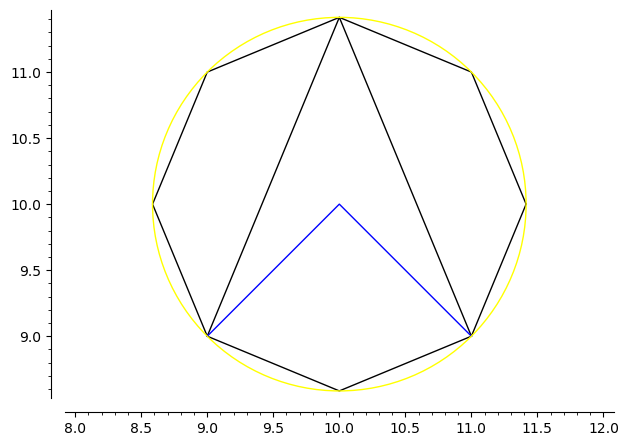
\includegraphics[scale=0.4]{octagon.png}

\end{enumerate}


% グラフはsagemathにて描画
% https://sagecell.sagemath.org/
%
%c=circle((10,10), sqrt(2), color='yellow')
%l1=line([(sqrt(2)+10,0+10), (1+10, 1+10), (0+10,sqrt(2)+10), (-1+10, 1+10),
%        (-sqrt(2)+10,0+10), (-1+10, -1+10), (0+10, -sqrt(2)+10), (1+10, -1+10),
%        (sqrt(2)+10,0+10)], color='black')
%l2=line([(-1+10,-1+10), (0+10,sqrt(2)+10), (1+10,-1+10)], color='black')
%l3=line([(-1+10,-1+10), (0+10,0+10), (1+10,-1+10)], color='blue')
%(c + l1 + l2 + l3).show(xmin=8, xmax=12)
%



\end{document}
